\chapter{Project Results}
\label{chp:results}
\lhead{Chapter \ref{chp:results}. \emph{Project Results}}

% TODO

\section{System Testing}

\FloatBarrier
\subsection{Board Level Testing}

During and after the construction phase of the robot's hardware, a number of verification tests were made to ensure that the various hardware modules were operating as expected. This step was critical in ensuring the correctness of the hardware before the main firmware was written, to rule out hardware errors in the software verification phase.

\FloatBarrier
\subsubsection{Main Power Supply}

The main power supply was tested with an oscilloscope, after the module components were installed onto the PCB. A static load of 300mA was placed on the switchmode supply output, and the voltage ripple on the supply measured with an oscilloscope (see Figure \ref{fig:mainpowerripple}). This yielded an output ripple of approximately 80mV, well within the tollerances of the system. At the given static load, the regulated output voltage was measured at 4.98V, within the specifictions of \(4.8V\leq\text{V\subscript{out}}\leq5.2V\) listed in the LM2595-5 regulator datasheet.

\begin{figure}[tbph]
	\vspace{1em}
	\centering
		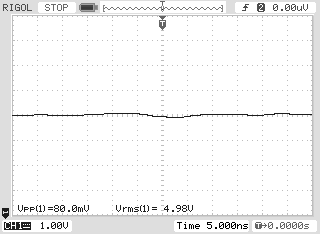
\includegraphics[width=90mm]{SM5V.png}
	\rule{35em}{0.5pt}
	\caption[Switch-mode 5V Power Supply Oscilloscope Trace]{Oscilloscope trace of the main 5V switchmode power supply showing ripple under static load.}
	\label{fig:mainpowerripple}
\end{figure}

\FloatBarrier
\subsubsection{Sensor Power Supply}

For the secondary 3.3V LDO power supply used by the board's sensor modules, an identical set of tests to those used in the verification of the main power supply were performed, using the sensor boards as the regulator output load. This yielded a ripple of 120mV, and an output voltage of 3.27V. When compared to the ADP3308 datasheet output's electrical characteristics, this was within the stated \(\pm1.2\%\) accuracy (\(3.26V\leq\text{V\subscript{out}}\leq3.34V\)).

\begin{figure}[tbph]
	\vspace{1em}
	\centering
		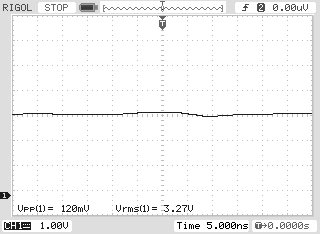
\includegraphics[width=90mm]{LDO3V.png}
	\rule{35em}{0.5pt}
	\caption[LDO 3.3V Power Supply Oscilloscope Trace]{Oscilloscope trace of the sensor 3.3V LDO power supply showing ripple under static load.}
	\label{fig:sensorpowerripple}
\end{figure}

\FloatBarrier
\subsubsection{Motor PWM Outputs}

To test the motor outputs (and, in turn, the entire motor controller circuit) the two motor output channels were connected to an oscilloscope in sequence, and a small test wrapper written over the motor driver firmware module. Each output was switched backwards and forwards at the maximum (safe) PWM rate, and the resulting waveforms verified against the expected waveforms. Figure \ref{fig:motorpwm} shows one such waveform, showing the left motor output at full speed.

\begin{figure}[tbph]
	\vspace{1em}
	\centering
		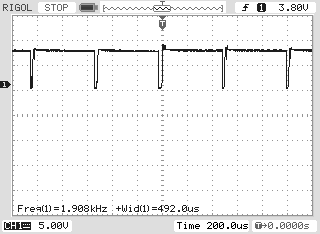
\includegraphics[width=90mm]{PWM.png}
	\rule{35em}{0.5pt}
	\caption[Motor PWM Oscilloscope Trace]{Oscilloscope trace of one motor channel PWM output while active, showing the frequency and duty cycle at full speed.}
	\label{fig:motorpwm}
\end{figure}

\FloatBarrier
\subsubsection{RGB Status LED}

A simple test routine was written to cycle through all possible colours on the mounted RGB status LED; this demonstrated that the three GPIO channels were configured and connected correctly, and that the appropriate brightness balancing for each sub-component in the LED package was set correctly by the chosen current limiting resistors on the board. As this is a simple but visually attractive piece of self-diagnostics, the test routine code was eventually retained in the final robot version during the robot's start-up sequence.

\FloatBarrier
\subsubsection{LCD and Backlight}

To test the board's LCD functions, a routine calling various formatting commands was written and wrapped around the completed LCD driver software module. These commands---containing various cursor placements, custom character definitions and formatted strings---indicated that the display was indeed working as expected. For the LCD backlight, code was written to slowly fade in the backlight brightness from the minimum value, up to the maximum in 10ms increments. Like the RGB LED test routine, this functionality was eventually incorporated into the start-up routine of the final robot firmware.

\FloatBarrier
\subsection{Software Testing}

% TODO

\section{Achieved Results}

% TODO

\begin{figure}[tbph]
	\vspace{1em}
	\centering
		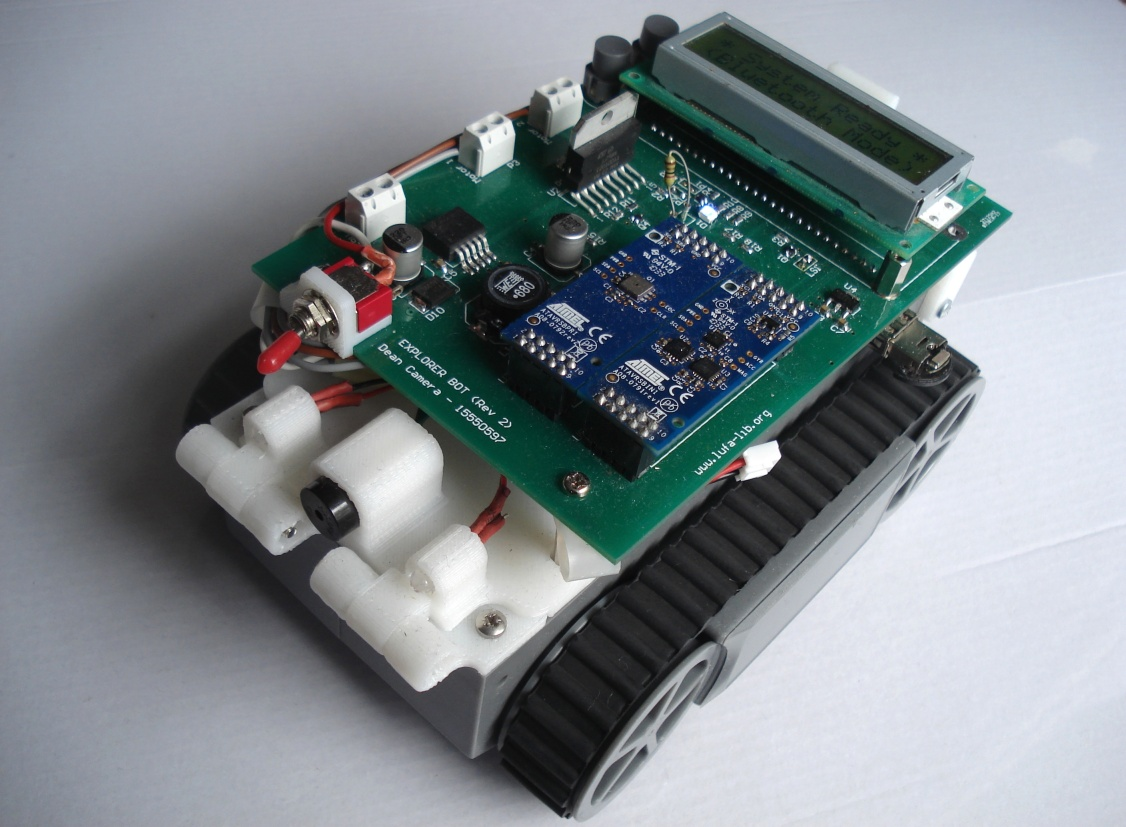
\includegraphics[width=140mm]{CompletedRobot.jpg}
	\rule{35em}{0.5pt}
	\caption[Photo of Completed Robot]{Photo of the completed \textit{ExplorerBot} prototype robot}
	\label{fig:completedrobot}
\end{figure}

\begin{figure}[tbph]
	\vspace{1em}
	\centering
		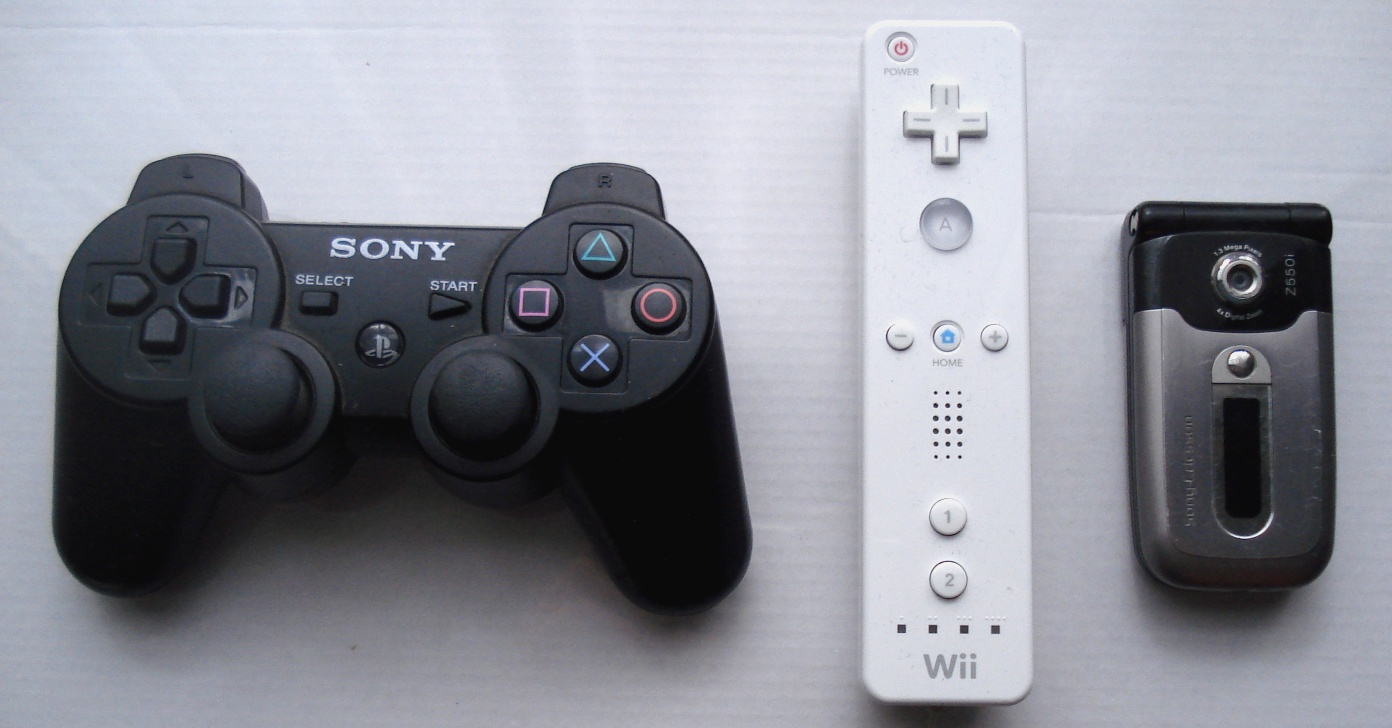
\includegraphics[width=140mm]{BluetoothControllers.jpg}
	\rule{35em}{0.5pt}
	\caption[Tested Working Controllers]{Tested consumer grade Bluetooth enabled devices: \\ Playstation 3 controller \textit{(left)}, Nintendo Wii controller \textit{(middle)}, Sony-Ericcson z550i mobile phone \textit{(right)} }
	\label{fig:workingbtcontrollers}
\end{figure}

\begin{figure}[tbph]
	\vspace{1em}
	\centering
		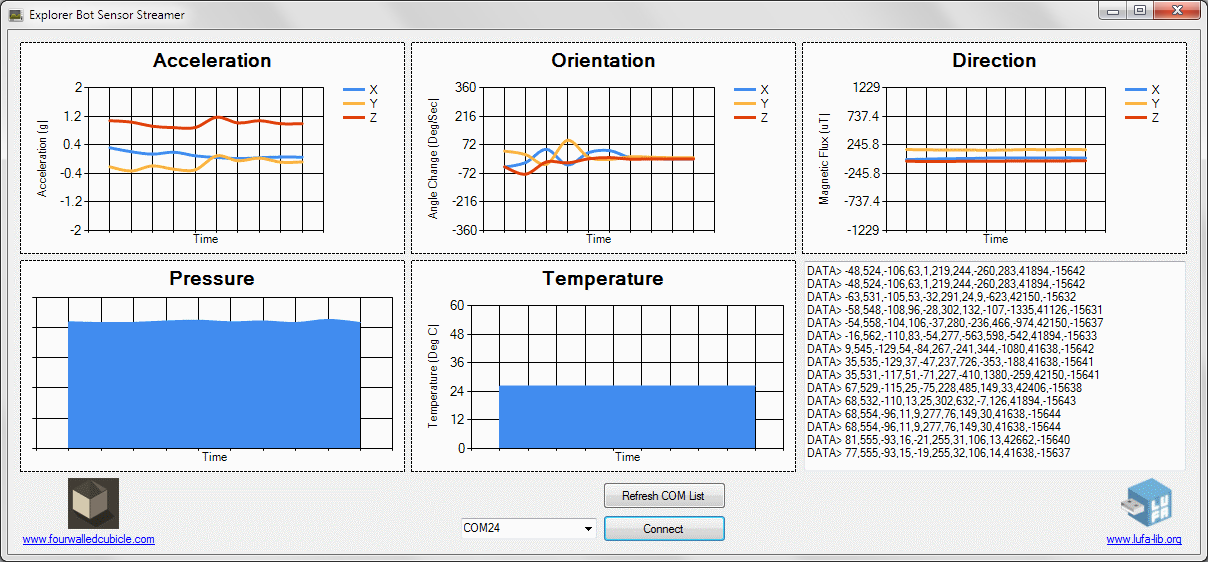
\includegraphics[width=140mm]{SensorDataApp.png}
	\rule{35em}{0.5pt}
	\caption[Sensor Logging Host Application]{Sensor logging application, showing data streaming wirelessly from the connected robot via a Bluetooth virtual serial port. }
	\label{fig:sensorhostapp}
\end{figure}
